\documentclass{exampaper}
\usepackage{graphicx, ulem, paralist, float, subfigure}

\examtitle{Minecraft红石等级测试}
\cotitle{二级 \qquad \uline{生}存用\uline{电}路}
\date{}

\begin{document}
    \maketitle

    % 注意事项
    \begin{material}
        \noindent \heiti 注意事项: \songti

        \begin{compactenum}
            \item 本卷满分100分,测试时间60分钟。
            \item 本卷中所有使用到的游戏特性均以Minecraft Java Edition 1.18.2版本为准。
            \item 本卷中所有设施运行结果均应当为其运行在$TPS=20.0$情况下的结果为准。
            \item 单位gt是gametick的缩写,1gt代表一个游戏刻。单位rt是redstonetick的缩写,代表一个红石刻,默认情况下$1rt=2gt$。单位ips是items per second的缩写,代表物品每秒。
            \item 上机操作题建议在服务器中完成,无法在服务器中完成的,可以提交上机操作的全程录屏。
            \item 上机操作题应当使用创造模式进行完成。
            \item 带有【Mod】标签的题目如因特殊原因无法完成,计一半分。
            \item 漏斗链运输的吞吐量为$2.5ips$。
        \end{compactenum}
    \end{material}

    % 30分
    \part{客观题}
        \section{选择题}{共6题,每题5分}
            \subsection{阅读如下材料,从下方四个选项中选择出正确答案。}
                \begin{material}
                    矿艺(Minecraft)(俗谓我的世界)者,电玩也。 可基方石、筑万物、建城邑、凿山河、引渠取矿,时以刻为计。 游戏之法,有创、生、极、勇、览诸道,戏者择其好而从之。 其无关卡之数,亦无时限,然乐以创世。 惟存道,需果腹、为室家。 嗣后,所行耑台甚众,且常赓之。—— 矿艺大典

                    矿艺之法,重于方石,亦有器具、实体。 戏者生于兹世,是谓主界; 斩木作材,猎呓为炙,以图生存。 然黑曜石,复孳焱界,业火异兽充于闲。 更坠终界之门,则入终界,鏖战于龙,得奇异珍。
                \end{material}

                \twoselections{终界代表下界}{终界代表末地}{Minecraft使用小时为单位进行计时}{Minecraft有3种游戏模式}

            \subsection{下面哪个因素影响刷怪塔的产出效率?}
                \twoselections{刷怪平台的高度}{当前的天气}{当前维度内村民的数量}{当前维度内铁傀儡的数量}
            
            \subsection{设一刷怪塔内怪物的平均存活时间为$t$,平均怪物量为$n$,平均每个怪物掉落$d$个物品,刷怪塔效率$P$(个物品/时间)应当表示为\dash{1cm}。}
                \twoselections{$P=d\cdot\frac{n}{t}$}{$P=dnt$}{$P=dn$}{$P=114514$}
            
            \subsection{已知不同维度间怪物的刷怪上限不互通,则可知\dash{1cm}的效率最高。}
                \twoselections{寻路刷怪塔}{仇恨吸引刷怪塔}{计时水流刷怪塔}{双维度刷怪塔}
            
            \clearpage

            \subsection{以下哪种方式可以最高效地获取铁锭?}
                \twoselections{流言刷铁机}{恐吓刷铁机}{自己挖矿}{找村民借点}

            \subsection{\textbf{【Mod】}Carpet模组为玩家提供了哪些功能?}
                \begin{compactenum}
                    \item 召唤假人。
                    \item 调节游戏速度。
                    \item 显示当前服务端的TPS和MSPT。
                    \item 方便管理员封禁玩家。
                \end{compactenum}

                \fourselections{1 3 4}{1 2 3}{2 3 4}{1 2 3 4}

    \part{主观题} % 30分
        \section{填空题}{共5题,每题2分} % 10分
            \subsection{红石中继器的输出信号为\dash{1cm}。}

            \subsection{对于一个产量$ips>5$的刷地毯机,使用\dash{2cm}运输才能将其的产物输送出。}

            \subsection{对于一个典型的红石非门,请你写出它的输入、输出对应表(真值表)。}

            \vspace{0.25cm}

            \begin{tabular}{|c|c|}
                \hline
                输入 & 输出 \\
                \hline
                关 & 开 \\
                \hline
                开 & \dash{1cm} \\
                \hline
            \end{tabular}

            \vspace{0.25cm}

            \subsection{如图,开启拉杆后,左侧的活塞将会\dash{1cm},右侧的活塞将会\dash{1cm}(填开启/关闭)。}

            \subsection{如图,请问中继器左侧的红石灯能否在整个夜间被激活。原因是\dash{4cm}。}

            % 图片区
            \begin{figure}[H]
                \subfigure[第9题图]{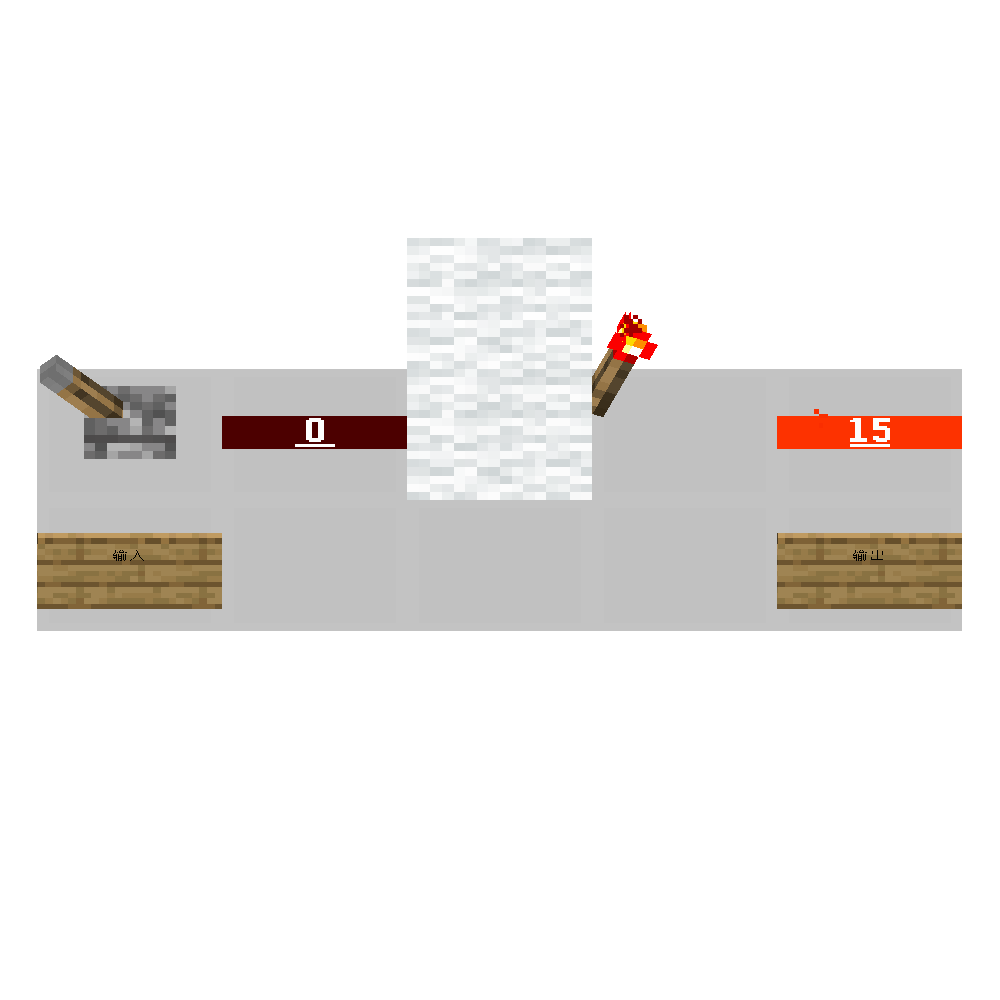
\includegraphics[width=3cm]{./images/L2/Q9.png}}
                \subfigure[第10题图]{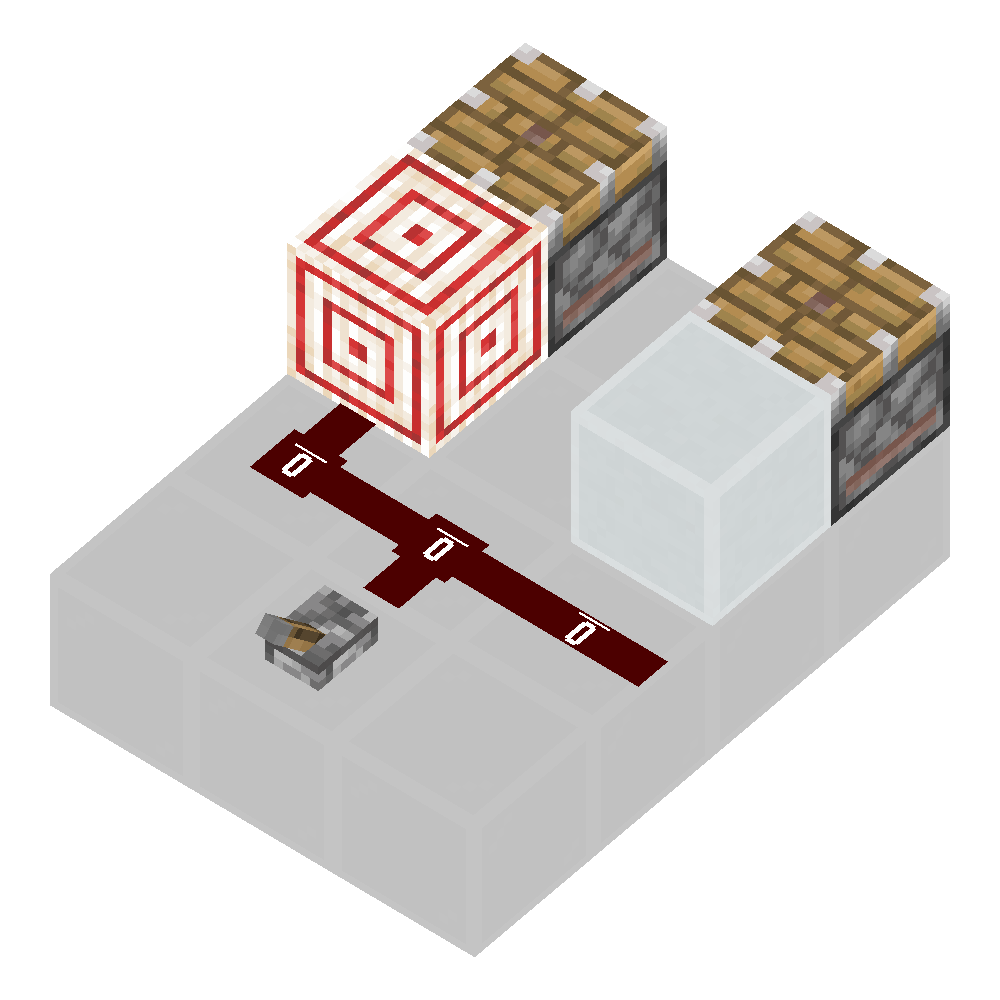
\includegraphics[width=3cm]{./images/L2/Q10.png}}
                \subfigure[第11题图]{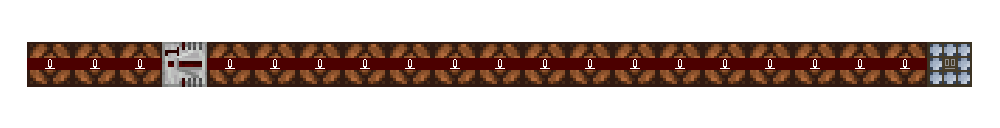
\includegraphics[width=8cm]{./images/L2/Q11.png}}
            \end{figure}
    
        \section{阅读材料,回答问题}{共2题,每题10分} % 20分
            \begin{material}
                \noindent \heiti 材料1: \fangsong

                陷阱箱可用于检测玩家何时打开了它的GUI。

                陷阱箱在不被打开时是没有信号的,但是当被玩家打开时会发出红石信号。从大型陷阱箱的任一部分打开都会使大型陷阱箱的两边都发出信号。生物无法打开陷阱箱,并且陷阱箱不会因为物品通过投掷器或漏斗被传送进来或出去而发出红石信号。

                当其被打开时,陷阱箱:

                \begin{compactitem}
                    \item 激活毗邻的红石粉,包括在陷阱箱下方的。信号等级等于正在使用陷阱箱的玩家数(最大为15)。
                    \item 激活任何背朝陷阱箱的红石中继器。
                    \item 给在其下方的红石导体强充能。充能等级等于正在使用陷阱箱的玩家数(最大为15)。
                    \item 激活任何毗邻的机械元件(除面向它的活塞外)。
                \end{compactitem}

                陷阱箱不会激活毗邻且背朝向它的红石比较器。红石比较器只能检测陷阱箱存储物品的数量。当比较器检测大型陷阱箱时,比较器会检测整个大型陷阱箱(54个槽位),而不只是比较器后方的那半个。无法打开的陷阱箱总会使比较器的检测信号为0,不受其中物品数量的影响。—— Minecraft Wiki

                \noindent \heiti 材料2: \fangsong

                丁字路口交叉处的弯道铁轨可以通过红石信号(譬如红石火把、拉杆等)改变其拐弯方向。

                \begin{figure}[H]
                    \centering
                        \subfigure{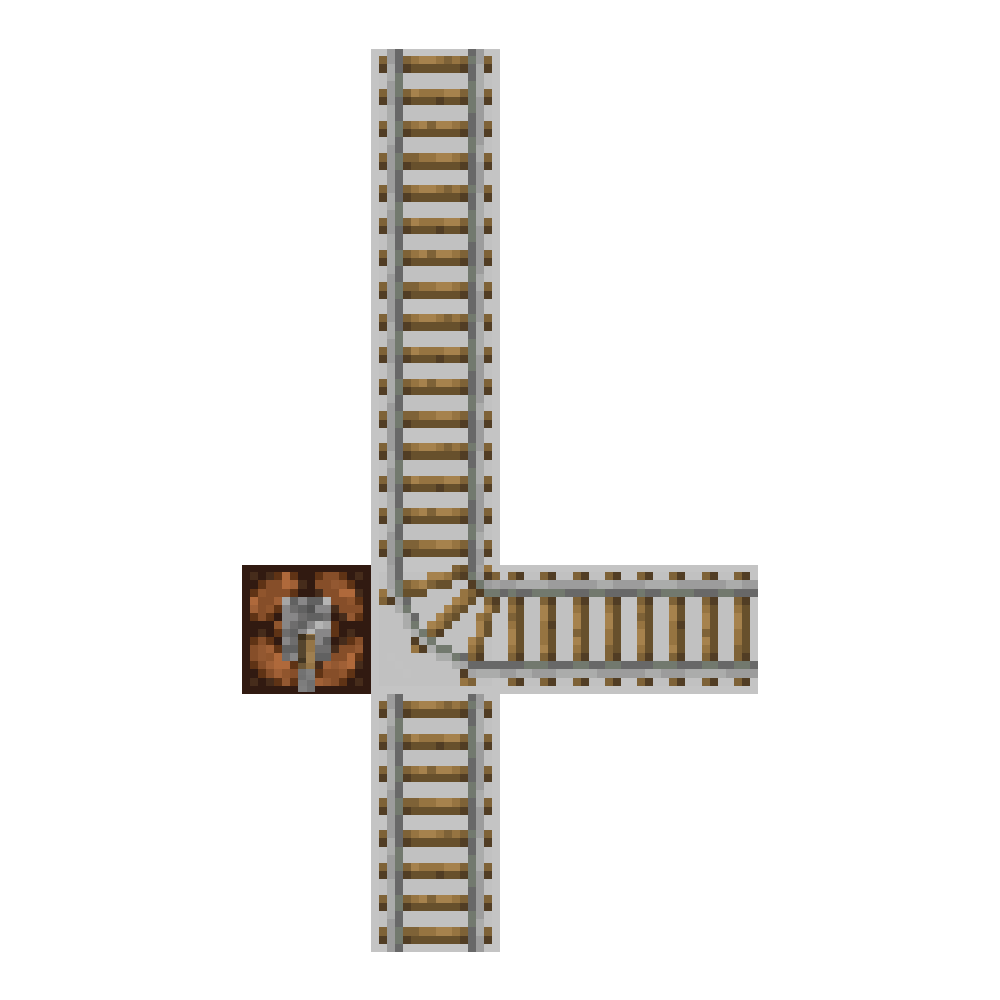
\includegraphics[width=3cm]{./images/L2/Material2-p1.png}}
                        \subfigure{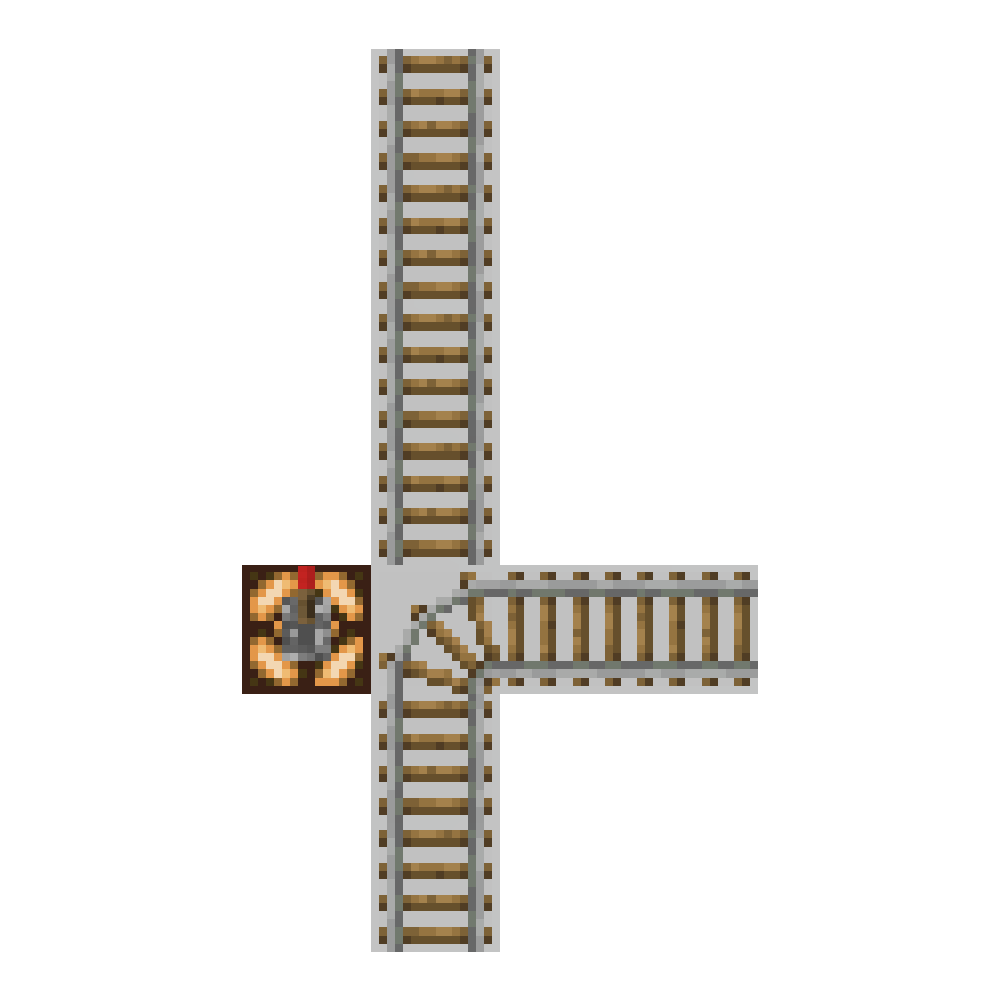
\includegraphics[width=3cm]{./images/L2/Material2-p2.png}}
                        \caption{材料2示例}
                \end{figure}
            \end{material}

            \subsection{请简要分析为何在很多服务器的铁路设施中,都使用陷阱箱来实现换向器,使得矿车可以在不同轨道间切换。}
                \vspace{2.5cm}
            
            \subsection{\textbf{【开放题】}利用陷阱箱的特性,设计一个陷阱,使得从陷阱箱中偷窃物品的人死亡并获取其背包中的所有物品。(死亡不掉落关闭)}
                \vspace{2.5cm}

    \clearpage

    \part{上机操作题} % 40分
        \section{运用所学知识,设计红石装置}{共5个评分点,每个评分点4分} % 20分
            \textbf{题目背景:}你正在游玩一个刚开服的生电服务器,目前服务器内十分缺乏铁锭,请你设计一个刷铁机,帮助服务器内的玩家获取铁锭。\textbf{要求使用潜影盒进行打包,以方便其他玩家取用。}
            
            \textbf{评分点如下:}

            \subsection{产出铁锭效率$\geq 200 items/hour$。}
            
            \subsection{刷铁机核心$\geq 2$核。}

            \subsection{自动过滤除铁锭外的副产物。}

            \subsection{\textbf{【Mod】}使用Carpet进行假人挂机。}

            \subsection{使用潜影盒进行打包。}

        \section{运用所学知识,改良红石装置}{共4个评分点,每个评分点5分} % 20分
            \textbf{题目背景:}某一生电服务器内有一刷石机,由于服务器内除你以外的玩家都不懂生电,因此该刷铁机的效率十分低下。经测定,该刷石机的效率为$60items/hour$,由于服务器内的一个工程需要大量圆石,因此其他玩家希望你改进刷石机。

            \textbf{评分点如下:}

            \subsection{产出圆石效率$\geq 120items/hour$。}

            \subsection{无需玩家或假人挂机,使用TNT复制模块(可上网搜索相关设计)炸圆石。}

            \subsection{保证TNT不会破坏其他结构。}

            \subsection{使用潜影盒进行打包。}
\end{document}